\begin{frame}[label=mc_investigation]
    \frametitle{\alert{Step 3:} Investigation}
    \begin{textblock*}{2cm}(\paperwidth-2.05cm, 0.05cm)
        \raggedleft 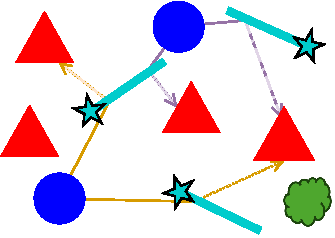
\includegraphics[height=1cm]{img/visible_sim.pdf}
    \end{textblock*}
    \begin{columns}
        \begin{column}{0.7\textwidth}
            \textit{What meteors are observed? For each meteor...}
            \begin{enumerate}
                \item Calculate signal-to-noise ratio: \(SNR = \frac{P_{RX}}{P_{noise}}\)
                \item Estimate probability of detection, \(P_{Detect}(SNR)\)
                \item Randomly determine observability based on \(P_{Detect}\)
            \end{enumerate}
        \end{column}
        \begin{column}{0.3\textwidth} 
            \centering 
            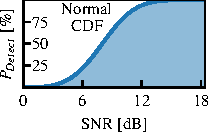
\includegraphics[width=0.5\linewidth]{img/param_distributions/P_detect.pdf}
        \end{column}
    \end{columns}
    ~ \\ ~ \\ 
    \hrule
    ~ \\ 
    \begin{columns}
        \begin{column}{0.7\textwidth}
            \alert{Area of coverage}: the ground area containing the majority of observations. \\ ~ \\
            
            \alert{Observation efficiency}: \(\eta = \frac{\text{\# observed}}{\text{\# generated}}\)
            \begin{itemize}
                \item[\(\blacktriangleright\)] Indicates how many meteors were missed 
                \item[\(\blacktriangleright\)] Helps answer: Are there 7x more meteors to see? 
            \end{itemize}
            %
            \alert{Observation density}: observed meteors per area per time 
            
            \alert{Observation counts}: total observations per time, \(\propto \text{Area} \times \eta\)
        \end{column}
        \begin{column}{0.3\textwidth}
            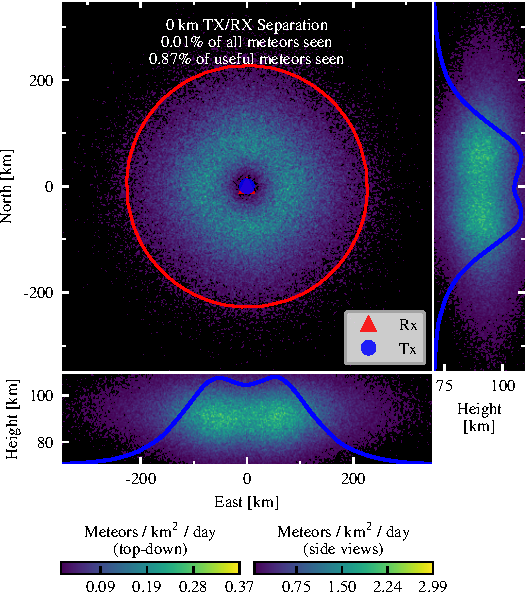
\includegraphics[width=\linewidth]{img/simulated_heatmap_0km.pdf}
        \end{column}
    \end{columns}
\end{frame}